\chapter{Isolas of localized structures and Raman–Kerr frequency combs in micro-structured resonators (Chaos, Solitons \& Fractals 174, 113808)}

In section~\ref{sec:fra_LS} we introduced the concept of dissipative 
localized structures (LSs) which can be observed in a huge variety
of systems including vegetation patterns, biology and 
nonlinear optics \cite{tlidi2014localized,heimburg2005soliton}. In the case of nonlinear optical systems,
a particularly interesting type of localized structure can be found,
the so-called optical solitons. Moreover, it has recently been discovered that the formation of solitons
in both fiber and micro-resonators gives rise to frequency combs, which are equally
spaced spectral lines. These frequency combs are remarkable
for technological purposes such as chip-scale atomic clocks \cite{Jost2015clock}, terabit
per second communication \cite{marin2017microresonator} and even the calibration of spectrometers
for exoplanet search \cite{suh2019searching}. From a theoretical perspective, the dynamics
of solitons in these optical resonator systems can be accurately described 
by the paradigmatic Lugiato-Lefever equation (LLE) \cite{lugiatolefever1987}.

In this chapter, we will study the formation of such structures in the
case of short solitons where the influence of the stimulated Raman scattering (SRS)
cannot be neglected and higher-order dispersion terms appear. In this case, a reduced model
in the form of a non-local Swift-Hohenberg equation is proposed to provide an
in-depth description and some analytical results. Employing a combination of
numerical simulations and
continuation of the reduced model (see \ref{sec:cont_traveling} for a detailed discussion on the
continuation of traveling states), we show that the SRS induces a forced symmetry
breaking leading to the motion of both the bright and dark solitons, as well as a disconnection between 
the different branches of LSs. Consequently, the traditional snaking bifurcation scenario breaks
apart and instead, a family of isolas appears. Lastly, a numerical analysis of the
original model, the generalized LLE, confirms the formation of isolas of drifting LSs due
to the reflection symmetry breaking, in agreement with previous studies \cite{burke2009swift,parra2014third}.

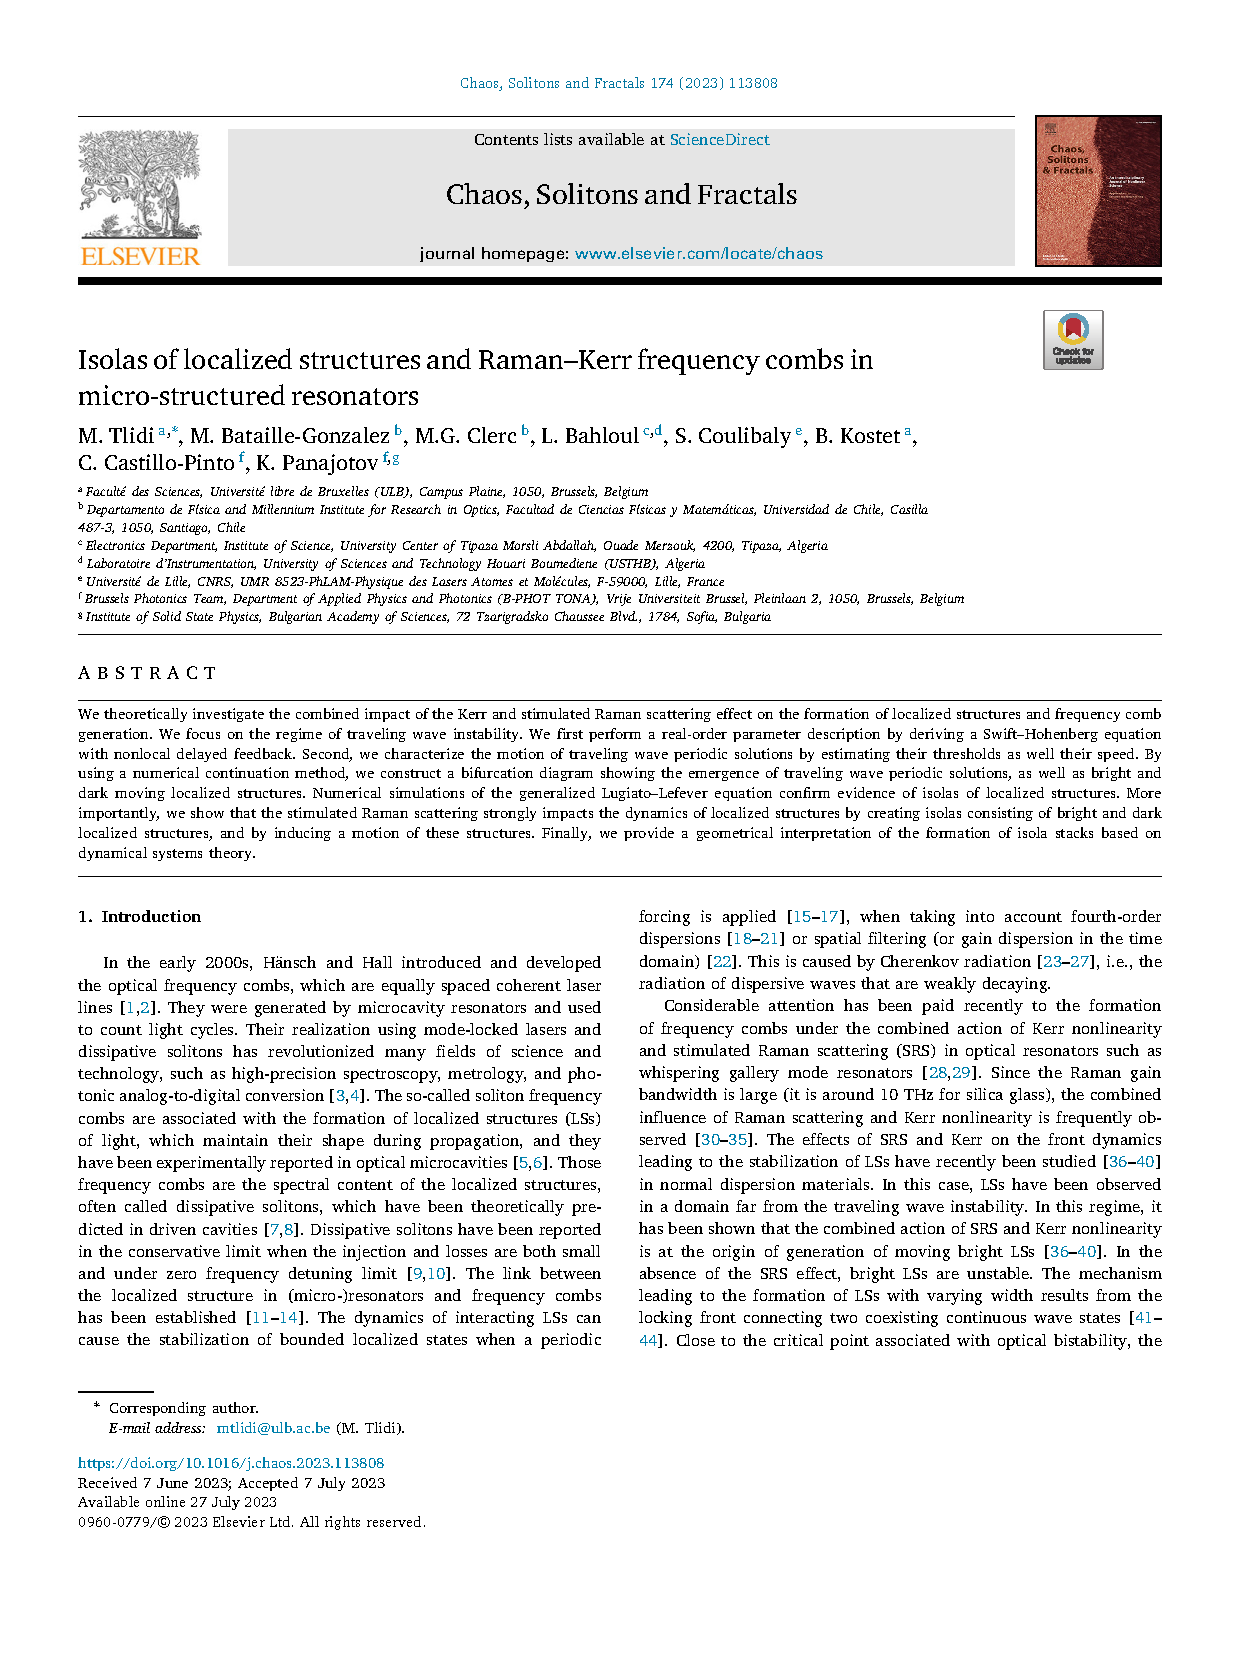
\includepdf[pages={-}]{chapters/isolas.pdf}

\section{Perspectives}

In this work, we have performed a detailed numerical analysis of the formation
of bright and dark solitons in a reduced non-local Swift-Hohenberg equation. More specifically,
we investigated the effect of a reflection symmetry-breaking term: the Raman effect on 
the LSs and summarized these results in a bifurcation diagram. Nevertheless, some bifurcations
present in the diagram were not completely characterized and should be studied further. 
For instance, the traveling 
wave and some LSs lose stability before the saddle-node bifurcation at an unidentified
bifurcation point. On the other hand, although we have successfully confirmed the main results
on the original model, a more complete bifurcation diagram, showing the stability and all of the LSs, 
remains
to be produced.
